本章的目的有两个。\footnote{原文为“本章的目的是双重的。”,机翻味太浓了(乐}首先将经典力学表示成,使经典力学和量子力学之间的联系显明的那样形式。

第二个目的是学习掌握量子化学中重要的二力学问题,即分子的振动和转动。这两种分子运动是红外和微波光谱学的核心。

开始一节是复习和一些定义,由此进到拉格朗日方程和哈密尔顿方程,以强调出与量子力学的联系,用对分子运动的应用来结束。

\section{导言和守恒定律}
在讨论经典力学时,将不受拘東地使用向量。我们生活和进行实验的世界是三维欧氏向量空间,因此可很快地将此空间的向量的性质概括如下:

(a)一向量$\mathbf{V}$通常可表示为笛卡儿基底的三个实分量
\[\mathbf{v}=(\mathbf{v}_x,\mathbf{v}_y,\mathbf{v}_z)=v_x\hat{x}+v_y\hat{y}+v_z\hat{z} \tag{4-1}\]
在本章中向量用通常的符号并以粗体字表示。单位向量用长音符号($\hat{ \quad }$)标记

(b)二向量的点积或标量积是
\[\mathbf{v}_1 \cdot \mathbf{v}_2=v_{1x}v_{2x}+v_{1y}v_{2y}+v_{1z}v_{2z} \tag{4-2}\]
它与第三章中称之为内积的量完全相同,类似地,向量$\mathbf{v}$的长度是$\sqrt{\mathbf{v} \cdot \mathbf{v}}$;如点积为零,则二向量垂直。

在力学中还定义另一类向量积。
\begin{definition}[叉积]
    定义二向量的叉积为
    \footnote{我个人感觉下面这种表达方式更清晰
    \[\mathbf{v}_1 \times \mathbf{v}_2=
    \begin{vmatrix}
        \hat{x} & \hat{y} & \hat{z} \\
        v_{1x} & v_{1y} & v_{1z} \\
        v_{2x} & v_{2y} & v_{2z}
    \end{vmatrix}
    \]}
    \[\mathbf{v_1} \times \mathbf{v_2}=(v_{1y}v_{2z}-v_{1z}v_{2y})\hat{x}+(v_{1z}v_{2x}-v_{1x}v_{2z})\hat{y}+(v_{x}v_{2y}-v_{1y}v_{2x})\hat{z} \tag{4-3}\]
\end{definition}

应注意,二向量的叉积给出一向量,而二向量的点积给出一标量。如向量的全部分量皆彼此可对易,则向量与自身的叉积$\mathbf{v} \times \mathbf{v}$为零。
如分量都是数,它们显然是可对易的,因而$\mathbf{v} \times \mathbf{v}=0$;但如果分量是算符,则需要应用算符的对易规则求$\mathbf{v} \times \mathbf{v}$。

本章的全部讨论都是从一些定义和牛顿定律出发。不考虑相对论效应。从讨论一质点开始并给出二定义。
\begin{definition}[动量]
    一质点的直线动量(或简称动量)是
    \[\mathbf{P}=m\mathbf{v} \tag{4-4}\]
    式中$m$是质点的质量,$\mathbf{v}$是速度\footnote{原书速度用$\mathbf{V}$表示,会与势能符号冲突,故此处及之后均改为小写$\mathbf{v}$。},$\mathbf{P}$是动量。
\end{definition}

\begin{definition}[角动量]
    一质点绕一点的角动量是
    \[\mathbf{l}=\mathbf{r} \times \mathbf{P} \tag{4-5}\]
    式中$\mathbf{r}$是质点与该点的距离向量$\mathbf{P}$是质点的(直线)动量,$\mathbf{l}$是角动量。
\end{definition}

为了简化符号,用点表示对时间的导数。这样,$\dot{\mathbf{r}}=\dv*{\mathbf{r}}{t}=\mathbf{v}$;$\dot{\mathbf{v}}=\dv*{\mathbf{v}}{t}=\mathbf{a}$(加速度)等等。牛顿第二定律表示为
\[\mathbf{F}=\dot{\mathbf{P}} \tag{4-6}\]
如果质量是常数,则这个非常简练的方程和人们熟悉的$\mathbf{F}=m\mathbf{a}$是等价的,因为$\mathbf{F}=\dv*{(m\mathbf{v})}{t}=m(\dv*{\mathbf{v}}{t})=m\mathbf{a}$。
简单的方程4-6实际上包含着相当于牛顿第一定律的守恒定理。

\begin{theorem}
    若作用于一质点上的合力为零,则质点的(直线)动量不随时间改变,或动量守恒。
\end{theorem}

我们可以问,对角动量是否也存在同样的守恒定理。可用$\mathbf{r}$(与点的距离向量)叉乘方程4-6的两边以证明此定理。
\[\mathbf{r} \times \mathbf{F}=\mathbf{r} \times \dot{\mathbf{P}}=r \times \dv{t}(m\mathbf{v}) \tag{4-7}\]
而
\[\dv{t}\left(\mathbf{r} \times m \mathbf{v}\right)=\mathbf{v} \times m \mathbf{v}+\mathbf{r} \times \dv{t}(m \mathbf{v})=\mathbf{v} \times m \mathbf{v}+\mathbf{r} \times \mathbf{P} \tag{4-8}\]
因$\mathbf{v} \times \mathbf{v}=0$,所以
\[\mathbf{r} \times \mathbf{F}=\dv{t}(\mathbf{r} \times \mathbf{P})=\dot{\mathbf{l}} \tag{4-9}\]
方程4-9的实质可用一定义和一定理概括。

\begin{definition}[转矩]
    施于绕一点的质点的转矩为
    \[\mathbf{N}=\mathbf{r} \times \mathbf{F} \tag{4-10}\]
    式中$r$是质点与该点的距离向量,$\mathbf{F}$是合力,$\mathbf{N}$是转矩。 
\end{definition}

\begin{theorem}
    若施于绕一点的质点的总转矩为零,则绕该点的角动量守恒(不随时间改变)。
\end{theorem}

对一个质点体系的最后一个守恒定理是涉及能量的,用两个定义来表示。

\begin{definition}[功]
    一质点移动距离$\dd{\mathbf{S}}$所作的功是
    \[\dd{W}=\mathbf{F} \cdot \dd{\mathbf{S}} \tag{4-11}\]
\end{definition}

\begin{definition}[保守力]
    保守力是这样一个力,它可与一标量势的负导数相联系:
    \footnote{原书的脚注:符号$\nabla$读着del或nabla,是向量微分算符:
    \[\nabla=+\frac{\partial v}{\partial x}\hat{x}+\frac{\partial v}{\partial y}\hat{y}+\frac{\partial v}{\partial z}\hat{z}\]
    $\nabla$作用于一标量给出向量,梯度,简写为grad。$\nabla$作用于向量有两种形式: 
    $\nabla \cdot \mathbf{a}=\text{div} \ \mathbf{a}$,称为$\mathbf{a}$的散度,是一标量;
    $\nabla \times \mathbf{a}=\text{curl} \ \mathbf{a}$,称为$\mathbf{a}$的旋度,为一向量。
    $\nabla \cdot \nabla$或$\nabla^2$称为拉普拉斯算符。
    对力学,电学,磁学做微底讨论时使用这些符号,而本章只偶而用到。}
    \[\mathbf{F}=-\frac{\partial v}{\partial x}\hat{x}-\frac{\partial v}{\partial y}\hat{y}-\frac{\partial v}{\partial z}\hat{z}=-\nabla v=-\text{grad} \ v \tag{4-12}\]
\end{definition}

可用这些定义计算一质点从点1移到点2所需之功。
\[W_{12}=\int_{(1)}^{(2)}\mathbf{F} \cdot \dd{\mathbf{S}}=\int F_x\dd{x}+\int F_y\dd{y}+\int F_z\dd{z}\]
\[=-\int\frac{\partial v}{\partial x}\hat{x}-\int\frac{\partial v}{\partial y}\hat{y}-\int\frac{\partial v}{\partial z}\hat{z}=-V_2-(-V_1)=V_1-V_2 \tag{4-13}\]
另一方面,因$\mathbf{F}=\dot{\mathbf{P}}=m\dot{\mathbf{v}}$,以及$\dd{\mathbf{S}}=\mathbf{v}\dd{t}$,也可得到
\[W_{12}=\int_{(1)}^{(2)}m\dot{\mathbf{v}} \cdot \mathbf{v}\dd{t}=\frac{m}{2}\int\dv{t}(\mathbf{v} \cdot \mathbf{v})\dd{t}=\frac{m}{2}\int\dv{(v^2)}{t}\dd{t}=\eval{\frac{mv^2}{2}}_{(1)}^{(2)}=\frac{m}{2}(v_2^2-v_1^2) \tag{4-14}\]
$mv^2/2$是动能,可用符号$T$表示;因而
\[W_{12}=T_2-T_1=V_1-V_2 \tag{4-15}\]
由此可得
\[T_2+V_2=T_1+V_1 \tag{4-16}\]
我们证明了下列定理

\begin{theorem}
    在保守力引起的运动中,能量$(T+V)$守恒。
\end{theorem}

到此为止只讨论了一个质点的体系。如果我们认同一些附加的定义,则这种分析可直接推广到多质点体系。
\begin{definition}[多质点体系]
    (a)作用于多质点体系中第$i$个质点上的总力是由两
    部分组成的,$\mathbf{F}^{out}_{i}$与\footnote{原书这里是$\mathbf{F}^{out}_{ij}$,不知道是少了个$\sum$还是多了个$_j$,应该是多了个$_j$。}质点内力的和
    \[\sum_{i \neq j}\mathbf{F}^{in}_{ij}\]
    牛顿第三定律给出$\mathbf{F}_{ij}=-\mathbf{F}_{ji}$。
    
    (b)质心的位置由向量
    \[\mathbf{R}=\frac{\sum_im_i\mathbf{r}_i}{\sum_im_i} \tag{4-17}\]
    确定,式中$m_i$是第$i$个质点的质量;$\mathbf{r}_i$是第$i$个质点的位置向量。
    
    (c) 体系的总质量为\[M=\sum_im_i\]
    
    (d)质心的动量是$\mathbf{P}=M\dot{\mathbf{R}}$
    
    (e)质心的角动量是$\mathbf{L}=\mathbf{R} \times \mathbf{P}$
\end{definition}

这五个定义容许有与前边三个定理类似的三个定理,也容许三个分离的定理,这些定理虽然重要,但还是只陈述不证明。
\begin{theorem}
    (a)若作用于多质点体系的总外力为零,则总(直线)动量守恒。\\
    (b)若作用于绕一点运动的多质点体系的总外转矩为零,则总角动量守恒。\\
    (c)若外加和质点内力二者皆是保守的,则能量$(T+V)$守恒。
\end{theorem}

下列的分离定理,证明整个体系是如何被分离成两部分的。
\begin{theorem}
    (a)多质点体系的总直线动量等于位于质心质量为$M$的一个质点的直线动量。\\
    (b)绕一点运动的多质点体系的总角动量等于质量为$M$的一个质点绕该点的角动量加上质点绕质心的角动量。\\
    (c)多质点体系的动能等于质量为$M$的一个质点以质心的速度$(\dot{\mathbf{R}})$运动的动能加上质点相对于质心的动能。
\end{theorem}

作者在本节和以后几节中都得助于几本完备的教科书,特别Goldslein的书。有兴趣的读者可从那些书中找到上述定理的证明。
这六个证明不特别难,它们将出现在本章末的习题中。

在本节里我们从改造牛顿定律为动量$\mathbf{P}$,角动量$\mathbf{l}$,和总能量$T+V$的守恒定理开始学习了经典力学。

\section{广义坐标和拉格朗日方程;哈密顿方程}
在本节中牛顿定律将被推导成具有二特殊有用性质的形式:这些方程是标量方程而非向量方程,这些方程可适用于任何坐标系。
到目前为止我们讨论了运动方程和守恒定理。除能量守恒定理外,都是特殊参考笛卡儿坐标系的向量方程。

无论在经典力学中还是在量子力学中,解物理或化学问题的一个决窍是根据问题的对称性明智地选择坐标系。
例如,地球绕太阳的运动(开普勒问题),在笛卡儿坐标中很难描述,但在球极坐标中就很自然。
电子绕核的运动(量子力学的氢原子问题),在笛卡儿坐标中很难对付,但在球极坐标中就直接了当。
将一体系的运动方程置于明智选择的坐标系中而得到的优越性是巨大的;同学们可能也感到掌握标量比掌握向量容易。
当然,在考察力学问题时,我们希望绝对的一般化。只能在球极坐标中建立运动方程是不够的:我们期望在一般化的坐标系中建立运动方程,因而选择的任何具体坐标系是完全一般化的坐标系的特例。
\begin{definition}[广义坐标]
    \textbf{广义坐标} \quad 描述$n$个质点的力学所需的$3n$个笛卡儿坐标的$3n$个坐标;都可表示为$3n$个广义坐标$q_i$和时间的函数:
    \[
    \begin{array}{c}
        x_1=x_1(q_1,q_2,\cdots,q_{3n},t) \\
        y_1=y_1(q_1,q_2,\cdots,q_{3n},t) \\
        \vdots \\
        z_n=z_n(q_1,q_2,\cdots,q_{3n},t) 
    \end{array}    
    \tag{4-18}
    \]
\end{definition}

一般化的位置向量用$\mathbf{r}_i$表示,$\mathbf{r}_i=(x_i,y_i,z_i)$。
在方程4-18中显函时间,因为坐标系可能移动,但在以后的讨论中时间不出现。

现在开始用牛顿第二定律(方程4-6)推导多质点休系的运动方程。对每个质点下式成立:
\[\mathbf{F}_i=\dot{\mathbf{P}}_i \tag{4-6}\]
推导从功的陈述开始。立刻得出一标量。质点$i$移动无限小距离$\delta \mathbf{r}_i$所作的功是
\footnote{原书的脚注:我们可以考虑压力所做的功,在最常见的情况下,压力的方向垂直于运动的方向;因而它做的功为零。我们讨论的情况正是这样。}
\[\mathbf{F}_i \cdot \delta \mathbf{r}_i=\dot{\mathbf{P}}_i \cdot \delta \mathbf{r}_i \tag{4-19}\]
应用变换方程4-18,为了简化去掉显函的时间变量。
\[\mathbf{r}_i=\mathbf{r}_i(q_1,\cdots,q_{3n}) \tag{4-20a}\]
\[\mathbf{v}_i=\dot{\mathbf{r}}_i=\sum_{k=1}^{3n}\frac{\partial \mathbf{r}_i}{\partial q_k}\dv{q_k}{t}=\sum_{k=1}^{3n}\frac{\partial \mathbf{r}_i}{\partial q_k}\dot{q_k} \tag{4-20b}\]
\[\delta \mathbf{r}_i=\sum_{k=1}^{3n}\frac{\partial \mathbf{r}_i}{\partial q_k}\delta q_k \tag{4-20c}\]
将方程4-19的左端用广义坐标表示并对全部质点求和得到
\[\sum_{i=1}^n\mathbf{F}_i \cdot \delta \mathbf{r}_i=\sum_{i=1}^n\sum_{j=1}^{3n}\mathbf{F}_i \cdot \frac{\partial \mathbf{r}_i}{\partial q_j}\delta q_j= \sum_{j=1}^{3n}Q_j\delta q_j \tag{4-21}\]
提醒一句:方程4-21中的两种求和范围不同,因为有n个质点,而广义坐标是3n个。
在方程4-21中出现的$Q_j$是什么?方程4-21的左端和右端有某些平行关系,因而促使我们提出下面的定义。

\begin{definition}[广义力]
    广义力$Q_j$是对应于广义坐标$q_j$的标量,定义为
    \[Q_j=\sum_{i=1}^n\mathbf{F}_i \cdot \frac{\partial \mathbf{r}_i}{\partial q_j} \tag{4-22}\]
\end{definition}

方程4-21的两端都具有(某种力)$\times$(某种坐标)这一形式。剩下方程4-19的右端需要讨论,它是比较难的。从二简单的陈述开始,这里不证明而留做习题。
\[\dv{t}\left(\frac{\partial \mathbf{r}_i}{\partial q_j}\right)=\frac{\partial \mathbf{v}_i}{\partial q_j} \tag{4-23a}\]
\[\frac{\partial \mathbf{r}_i}{\partial q_j}=\frac{\partial \mathbf{v}_i}{\partial \dot{q}_j} \tag{4-23b}\]
而
\[\sum_i\dot{\mathbf{P}}_i \cdot \delta \mathbf{r}_i=\sum_im_i\ddot{\mathbf{r}}_i\cdot \delta \mathbf{r}_i=\sum_im_i\ddot{\mathbf{r}}_i\cdot\sum_j\frac{\partial \mathbf{r}_i}{\partial q_j}\delta q_j\]
\[=\sum_{ij}\left(\dv{t}\left(m_i\dot{\mathbf{r}}_i\cdot \frac{\partial \mathbf{r}_i}{\partial q_j}\right)-m_i\dot{\mathbf{r}}_i\cdot \dv{t}\frac{\partial \mathbf{r}_i}{\partial q_j}\right)\delta q_j \tag{4-24}\]
将方程4-23代入,可得
\[\sum_i\dot{\mathbf{P}}_i \cdot \delta \mathbf{r}_i=\sum_{ij}\left(\dv{t}\left(m_i\mathbf{v}_i\cdot \frac{\partial \mathbf{v}_i}{\partial \dot{q}_j}\right)-m_i\mathbf{v}_i \cdot \frac{\partial \mathbf{v}_i}{\partial q_j}\right)\delta q_j\]
\[=\sum_j\left(\dv{t}\left(\frac{\partial}{\partial \dot{q}_j}\sum_i\frac{m_iv_i^2}{2}\right)-\frac{\partial}{\partial q_j}\sum_i\frac{m_iv_i^2}{2}\right)\delta q_j=\sum_j\left(\dv{t}\frac{\partial T}{\partial \dot{q}_j}-\frac{\partial T}{\partial q_j}\right)\delta q_j \tag{4-25}\]
因$T=\sum m_iv_i^2/2$。这样就将方程4-19右端约化为含标量和广义坐标的形式。
方程4-21和4-25二式都有对位移$\delta q_j$的求和。因广义坐标是独立的,故方程4-21和4-25可逐项比较。因此,将方程4-25和4-21结合起来可建立下列定理。

\begin{theorem}[拉格朗日方程的第一个形式]
在$3n$个广义坐标中的
含$n$个质点体系的运动方程是取下列形式的$3n$个方程
\[\dv{t}\frac{\partial T}{\partial \dot{q}_j}-\frac{\partial T}{\partial q_j}=Q_j \tag{4-26}\]
$j=1, \cdots ,3n$,$Q_j$是方程4-22的广义力,$T$是动能。
\end{theorem}

为了完成对广义坐标中经典力学的讨论,返回来讨论广义力。
正如能够用动能$T$表示$\dot{\mathbf{P}}_i \cdot \delta \mathbf{r}_i$项那样,我们也能够用势能$V$表示$Q_j$,从而达到在方程美的对称性要求。
方程4-22给出$Q_j$的定义。如果其中出现的$F_j$是保守的,则可将它写成势能的导数(方程4-12)。合并方程4-12和4-22,可得
\[Q_j=\sum_{i=1}^n\mathbf{F}_i \cdot \frac{\partial \mathbf{r}_i}{\partial q_j}
=\sum_{i=1}^n\left(F_{ix}\frac{\partial x_i}{\partial q_j}+F_{iy}\frac{\partial y_i}{\partial q_j}+F_{iz}\frac{\partial z_i}{\partial q_j}\right)\]
\[=-\sum_{i=1}^n\left(\frac{\partial v}{\partial x_i}\frac{\partial x_i}{\partial q_j}+\frac{\partial v}{\partial y_i}\frac{\partial y_i}{\partial q_j}+\frac{\partial v}{\partial z_i}\frac{\partial z_i}{\partial q_j}\right)=-\frac{\partial v}{\partial q_j} \tag{4-27}\]
拉格朗日方程的第一个形式(方程4-26)变成
\[\dv{t}\frac{\partial T}{\partial \dot{q}_j}-\frac{\partial T}{\partial q_j}=-\frac{\partial v}{\partial q_j} \tag{4-28}\]
为了完成这些方程的对称结构,加上势能与速度无关这一限制条件
\footnote{原书的脚注:此限制条件不总是需要的, 但它可使讨论相当简化。Goldstein证明了这种限制可以避免。}
。因此,$\partial v/\partial \dot{q}_j=0$,方程 4-28可重新写为
\[\dv{t}\frac{\partial (T-V)}{\partial \dot{q}_j}-\frac{\partial (T-V)}{\partial q_j}=0 \tag{4-29}\]
由它直接引出一定义和拉格朗日第二个形式。

\begin{definition}[拉格朗日函数]
    拉格朗日函数是标量力学量,其定义为
    \[L=T-V \tag{4-30}\]
\end{definition}

\begin{theorem}[拉格朗日方程第二个形式]
    在$3n$个广义坐标中的$n$个质点体系的运动方程是具有下列形式的$3n$个方程
    \[\dv{t}\frac{\partial L}{\partial \dot{q}_j}-\frac{\partial L}{\partial q_j}=0 \tag{4-31}\]
    式中$L$是方程4-30定义的拉格朗日函数。
\end{theorem}

拉格朗日处理方法对确认运动守恒有帮助,即守恒定理的陈述有帮助。特别是我们找到了下列定理。
\begin{theorem}[广义守恒定理]
    若$\partial L/\partial q_j=0$,则力学量$\partial L/\partial \dot{q}_j$(广义动量)守恒。
\end{theorem}

做为拉格朗日处理方法的基础工作的简例,我们分析示于图4-1的滑轮与重物体系。

\begin{figure}[htbp]
    \centering
    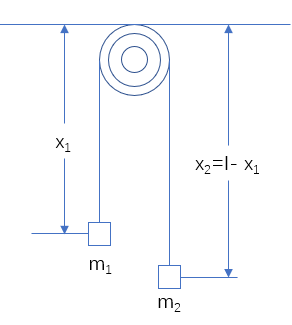
\includegraphics[scale=0.6]{./fig/4-1.png}
    \caption{阿德武德机,包括理想滑轮和二物体}
\end{figure}

\textbf{例}

示于图4-1的体系的质量为$m_1$和$m_2$二质点和无摩擦无重量的滑轮和拉绳,该体系用$F=ma$就能做分析。
但为了说明处理方法,我们用拉格朗日形式来处理。首先,求势能(产生于重力)
\[V=-m_1gx_1-m_2g(l-x_2)\]
式中$l$如图4-1所示。再求动能
\[T=\frac{1}{2}m_1\dot{x}_1^2+\frac{1}{2}m_2\dot{x}_2^2=\frac{1}{2}(m_1+m_2)\dot{x}_1^2\]
因$\dot{x}_1=-\dot{x}_2$。此广义坐标体系是单一坐标$x_1$体系。拉格朗日函数为
\[L=T-V=\frac{1}{2}(m_1+m_2)\dot{x}_1^2+g(m_1-m_2)x_1+m_2gl\]
我们要求算的拉格朗日方程为
\[\frac{\partial L}{\partial x_1}=(m_1-m_2)g\]
\[\frac{\partial L}{\partial \dot{x}_1}=(m_1+m_2)\dot{x}_1\]
因只有一个坐标,故也只有一拉格朗日方程,
\[\dv{t}(m_1+m_2)\dot{x}_1-(m_1-m_2)g=0\]
或
\[(m_1+m_2)\ddot{x}_1=(m_1-m_2)g\]
它与牛顿定律$F=ma$准确地等价。

本章末的习题将说明在牛顿方程比较笨拙的情况下的拉格朗日方程。

做为将牛顿定律表示为拉格朗日方程形式的结果,我们能够导出广义守恒定理:若$\partial L/\partial q_j=0$,则力学量$\partial L/\partial \dot{q_j}$(广义动量)守恒。
若用笛卡儿坐标表示$L$,
\[L=T-V=\frac{m}{2}(\dot{x}^2+\dot{y}^2+\dot{z}^2)-V(x,y,z) \tag{4-32}\]
则$\partial L/\partial x=F_x$,$x$方向的力,$\partial L/\partial \dot{x}=m\dot{x}=p_x$, x方向的动量。
这样,从拉格朗日形式的守恒定理又得出原来的动量守恒定理。我们也可以给出结构平行和权重相同的坐标(或位置)和动量以定义一广义动量。
\begin{definition}[广义动量]
    定义与广义坐标$q_i$共轭的广义动量$p_i$为
    \[p_i=\frac{\partial L}{\partial \dot{q}_i} \tag{4-33}\]
\end{definition}

用此定义,拉格朗日方程能够改写为
\[\dot{p}_i=\frac{\partial L}{\partial q_i} \tag{4-34}\]
用位置和动量来表示力学比单用位置表示其优点有二。
第一,现位置和动量之间的显著的平行结构,它在经典力学和量子力中都构成许多有意义的结果。
第二,可用$6n$个($3n$个$q$和$3n$个$p$)一阶微分方程表示的运动方程代替单用$3n$个($3n$个$q$)二阶微分方程。
即把位置和动量二者都看作是独立变量,这就使我们用两倍的方程式换来了数学上的简化。
为了做到这一点,即用$q's$和$p's$写运动方程,我们先定义一有巨大意义的新力学量。

\begin{definition}[哈密顿函数]
    含几个质点的体系的哈密顿函数为
    \[H=\sum_i p_i \cdot \dot{q}_i-L \tag{4-35}\]
\end{definition}

像前边考虑那样,广义坐标不显含时间,势能与速度无关,我们可以写出
\[\dd{H}=\sum_i\left(\frac{\partial H}{\partial q_i}dq_i+\frac{\partial H}{\partial p_i}dp_i\right) \tag{4-36}\]
由方程4-35得出
\[\frac{\partial H}{\partial q_i}=\sum_ip_i \cdot \frac{\partial \dot{q}_i}{\partial q_i}-\frac{\partial L}{\partial \dot{q}_i}\frac{\partial \dot{q}_i}{\partial q_i}-\frac{\partial L}{\partial q_i} \tag{4-37a}\]
\[\frac{\partial H}{\partial p_i}=\dot{q}_i \tag{4-37b}\]
因$\partial L/\partial \dot{q}_i=p_i$,$\partial L/\partial q_i=\dot{p}_i$,代入方程4-36,得到
\[\dd{H}=\sum_i\left(-\dot{p}_idq_i+\dot{q}_idp_i\right) \tag{4-38}\]
或
\[\dot{q}_i=\frac{\partial H}{\partial p_i} \qquad \dot{p}_i=-\frac{\partial H}{\partial q_i} \tag{4-39}\]
常称方程4-39为哈密顿方程。然而,哈密顿函数的性质是什么?
到目前为止我们只知道一抽象定义,方程4-35。$H$的一重要性质是,它是保守的,或在运动中守恒。
\[\dv{H}{t}=\sum_i\left(\frac{\partial H}{\partial q_i}\dot{q}_i+\frac{\partial H}{\partial p_i}\dot{p}_i\right)+\frac{\partial H}{\partial t}=\sum_i\left(-\dot{p}_i\dot{q}_i+\dot{q}_i\dot{p}_i\right)+\frac{\partial H}{\partial t}=\frac{\partial H}{\partial t} \tag{4-40}\]
从方程可见,除非$H$显函时间,否则$H$与时间无关,或在运动中守恒。
最后,为了将$H$与常见的物理量联系起来,我们集中考察动能:
\[T=\frac{1}{2}\sum_im_iv_i^2=\frac{1}{2}\sum_im_i\left(\sum_j\frac{\partial \mathbf{r}_i}{\partial q_j}\dot{q}_j\right)^2 \tag{4-41}\]
若$\mathbf{r}$不显函时间,则
\[T=\frac{1}{2}\sum_im_i\sum_{jk}\frac{\partial \mathbf{r}_i}{\partial q_j} \cdot \frac{\partial \mathbf{r}_i}{\partial q_k}\dot{q}_j\dot{q}_k=\frac{1}{2}\sum_{jk}t_{jk}\dot{q}_j\dot{q}_k \tag{4-42}\]
式中
\[t_{jk}=\sum_im_i\frac{\partial \mathbf{r}_i}{\partial q_j} \cdot \frac{\partial \mathbf{r}_i}{\partial q_k} \tag{4-43}\]
由此可得
\[\frac{\partial T}{\partial \dot{q}_i}=\sum_kt_{ik}\dot{q}_k \tag{4-44}\]
因而,
\[\sum_i \dot{q}_i\frac{\partial T}{\partial \dot{q}_i}=2T \tag{4-45}\]
现在可援引广义动量的定义,方程4-34。若势能与速度无关则\footnote{原书下式第一个等号后的$L$,写成了$T$(笑}
\[p_i=\frac{\partial L}{\partial \dot{q}_i}=\frac{\partial T}{\partial \dot{q}_i} \tag{4-46}\]
最后,
\[H=\sum_ip_i\dot{q}_i-L=\sum_i\frac{\partial T}{\partial \dot{q}_i}\dot{q}_i-T+V=2T-T+V=T+V \tag{4-47}\]
或,对势能与速度无关的保守系,哈密顿函数是总能量。所有这些结果可用一个定理表示。
\begin{theorem}
对势能与速度无关的保守系,若哈密顿函数不显函时间,则它在运动中守恒,因此在此条件下(总)能量守恒。最后,若$H$不随(广义)坐标变,则与该坐标共轭的动量守恒;若$H$不随动量变,则与该动量共轭的坐标守恒。
\end{theorem}

我们引入最后一个定义做为经典力学中最后一个课题,它与哈密顿处理一起构成联结量子力学和经典力学的途径。
\begin{definition}[泊松括号]
    定义二力学量$F$和$G$的泊松括号为
    \[\{F,G\}=\sum_i\left (\frac{\partial F}{\partial q_i}\frac{\partial G}{\partial p_i}-\frac{\partial F}{\partial p_i}\frac{\partial G}{\partial q_i}\right ) \tag{4-48}\]    
\end{definition}
泊松括号的一个重要应用是它可以示出守恒性质,因
\[\dv{F}{t}=\frac{\partial F}{\partial t}+\sum_i\left(\frac{\partial F}{\partial q_i}\dot{q}_i+\frac{\partial F}{\partial p_i}\dot{p}_i\right)
=\frac{\partial F}{\partial t}+\sum_i\left (\frac{\partial F}{\partial q_i}\frac{\partial H}{\partial p_i}-\frac{\partial F}{\partial p_i}\frac{\partial H}{\partial q_i}\right )=\frac{\partial F}{\partial t}+\{F,H\} \tag{4-49}\]
因此,若$F$不显函时间,则在$F$和$H$的泊松括号为零的条件下$F$在运动中守恒。

在本节中我们介绍了经典力学的两种数学处理。

1.拉格朗日方程。用$3n$个广义坐标表示的$3n$个二阶微分方程:
\[\dv{t}\frac{\partial L}{\partial \dot{q}_i}-\frac{\partial L}{\partial q_i}=0\]

2.哈密顿方程。用$3n$个广义坐标和$3n$个广义动量表示的$6n$个一阶微分方程:
\[\frac{\partial H}{\partial p_i}=\dot{q}_i \qquad -\frac{\partial H}{\partial q_i}=\dot{p}_i\]

这些数学处理能帮助我们记认守恒定理。特别重要的一点是:不显函时间的哈密顿函数在运动中守恒。
在某种常见的情况下,哈密顿函数等于体系的总能量。第五章将示出哈密顿经典力学怎样才能与量子力学联系起来。

\section{力学体系的振动}
在本节中我们将用上节中发展的拉格朗日力学研究质点体系的振动。

$n$个质点的体系有$3n$个自由度;其中有$3$个移动自由度和$3$个转动自由度。
因此,有$3n-6$个振动自由度。对线形分子此简单计算需要修正,线形分子只有$2$个转动自由度,因而振动自由度是$3n-5$。

拉格朗日量是$L=T-V$。因此,需要将$T$和$V$用广义坐标写出。由方程4-42和4-43知
\[T=\frac{1}{2}\sum_{jk}t_{jk}\dot{q}_j\dot{q}_k \tag{4-42}\]
\[t_{jk}=\sum_im_i\frac{\partial \mathbf{r}_i}{\partial q_j} \cdot \frac{\partial \mathbf{r}_i}{\partial q_k} \tag{4-43}\]
$T$是广义速度的二次函数\footnote{原书公式后此句开头有个"或,",感觉句意不通删了。}。$T$还可以用矩阵元为数$t_{jk}$的矩阵表示。

一真实振动分子的势能是一个复杂的和未完全被了解的函数。
但当离开平衡位置的位移很小时,用谐振势能函数作力学体系的振动的简单计算,常常是对真实分子势能的良好近似。
具有这个势能的力学体系称为谐振子;此势能函数与描述服从虎克定律的质点体系的势能函数等同:
\[V=\frac{1}{2}\sum_{jk}v_{jk}q_jq_k \tag{4-50}\]
或,势能$V$是广义坐标的二次函数。$V$也可用其矩阵元为数$v_{jk}$的矩阵表示。

现在可以写出拉格朗日函数
\[L=T-V=\frac{1}{2}\sum_{jk}(t_{jk}\dot{q}_j\dot{q}_k-v_{jk}q_jq_k) \tag{4-51}\]
根据拉格朗日方程,方程4-31,
\[\dv{t}\frac{\partial L}{\partial \dot{q}_j}-\frac{\partial L}{\partial q_j}=0 \tag{4-31}\]
得出
\[\dv{t}\left(\frac{1}{2}\sum_kt_{jk}\dot{q}_k\right)+\frac{1}{2}\sum_kv_{jk}q_k=0\]
\[\sum_k(t_{jk}\ddot{q}_k+v_{jk}q_k)=0 \tag{4-52}\]
不出所料,此方程与简谐运动方程形式上相似;因此,可取尝试解为$q_k=\phi_k\sin\omega t$,$\phi_k$是振幅,$\omega$是振动频率。可得
\[\sum_k\left(v_{jk}\phi_k-\omega^2t_{jk}\phi_k\right)=0 \tag{4-53}\]
这正是变量为$\phi_k$的一组联立线性齐次方程,它有解\footnote{应该是非全零解。}的条件是系数行列式为零:
\[
\begin{vmatrix}
    v_{11}-\omega^2t_{11} & v_{12}-\omega^2t_{12} & \cdots & v_{1n}-\omega^2t_{1n} \\
    v_{21}-\omega^2t_{21} & v_{22}-\omega^2t_{22} & \cdots & v_{2n}-\omega^2t_{2n} \\
    \vdots & \vdots & \ddots & \vdots \\
    v_{n1}-\omega^2t_{n1} & v_{n2}-\omega^2t_{n2} & \cdots & v_{nn}-\omega^2t_{nn}
\end{vmatrix} 
=0 \tag{4-54}   
\]
此方程酷似方程3-82示出的算符的特征值的久期方程。虽然在主对角线上和主对角线以外的特征值都乘以动能矩阵T的矩阵元,但我们也可以将方程4-54叫久期方程。
它有与$\phi_{n'^s}$同样数目的$3n-6$(或$3n-5$)个根$\omega^2$。类似地,可将方程4-53中的方程组写成特征向量方程:
\[V\phi^i=\omega^2T\phi^i \tag{4-55}\]
即,$V$作用于$\phi^i$给出$T$作用于$\phi^i$的倍数($\omega_i^2$)。
\begin{theorem}
    特征值$\{\omega^2\}$必须是非负的和实的。
\end{theorem}

此定理可沿上一章给出的相同的路线加以证明。$\omega^2$是非负的就已充分了,因这样$\omega$必是实的。我们可用另一形式的定理回答分子振动的特征值问题。
\begin{theorem}
特征向量$\{\phi^i\}$形成的以$\{\phi^i\}$为列的矩阵$\Phi$通过下列变换可同时将$V$和$T$对角化:
\[\Phi'V\Phi=\Omega \tag{4-56a}\]
\[\Phi'T\Phi=E \tag{4-56a}\]
式中$\Omega$是其对角元为$\omega^2$的可能值的矩阵,E是单位矩阵。
\end{theorem}

这里的变换虽具有$\Phi'V\Phi$和$\Phi'T\Phi$的形式,但不是相相似变换。方程中的变换称为迭合变换\footnote{特征向量集是相互正交的,转置等于逆,所以这里说是相似变换也没问题。}。用矩阵$\Omega$和$\Phi$可将特征值方科4-55改写成
\[V\Phi=T\Phi\Omega \tag{4-57}\]
左乘$\Phi'$,得
\[\Phi'V\Phi=\Phi'T\Phi\Omega \tag{4-58}\]
将它与习用的特征值问题(如方程3-86)的对应结果比较。因$\Phi'$是正交的,故方程3-86可改写为
\[\Phi'Q\Phi=\Phi'\Phi\hat{q} \tag{3-86}\]
在方程4-58中,方程3-86的$\Phi'\Phi$被$\Phi'T\Phi$替代;这可与方程4-54和方程3-82之间的差别比较。
事实上,正如方程3-86中$\Phi'\Phi=E$(单位矩阵)那样,我们可以证明方程4-58中$\Phi'T\Phi$也是单位矩阵。
因为$\phi^j$对方程4-55的左乘内积为
\[\bra*{\phi^j}V\ket*{\phi^i}=\omega_i^2\bra*{\phi^j}T\ket*{\phi^i} \tag{4-59}\]
$\phi^j$右乘的内积为
\[\bra*{V\phi^i}\ket*{\phi^j}=\omega^2_j\bra*{T\phi^i}\ket*{\phi^j}\]
\[\bra*{\phi^j}\ket*{V\phi^i}=\omega^2_j\bra*{\phi^j}T\ket*{\phi^i} \tag{4-60}\]
故比较方程4-59和4-60,可得
\[(\omega_j^2-\omega_i^2)\bra*{\phi^j}T\ket*{\phi^i}=0 \tag{4-61}\]
或,因特征值不同$\omega_j^2 \neq \omega_i^2$,故$\bra*{\phi^j}T\ket*{\phi^i}=0$。最后,对向量$\{\phi^i\}$作适当地调整,我们可以得出对所有$\phi^j$ ,$\bra*{\phi^j}T\ket*{\phi^j}=1$。
这些陈述和在通常的特征值问题中特征向量的正交归一性类似。

因此,可以得出如方程4-56b那样,中$\Phi'T\Phi=E$,如方程4-56a那样,方程4-58变成$\Phi'V\Phi=\Omega$。

用一个说明如何将这种处理方法应用于分子振动的简单例子结束这一节。
应该在开始时就指出,比这里介绍的方法更复杂的方法也可以用,并且也已被用于复杂分子的振动。
但问题的一般特点及其解法是相同的。

\textbf{例}

有一分子只沿直线振动(这是实际不存在的简化)。如图4-2所示分子是对称的。
我们需要先求算在示出的坐标系(这只是做为例子——也可以选其它坐标系)中势能和动能,然后将势能和动能表示为矩阵。
先考虑势能。在作谐振子近似中势能用一些项表示,每一项是键扩张的平方乘虎克定律力常数:
\[V=\frac{k}{2}(x_2-x_1-b)^2+\frac{k}{2}(x_3-x_2-b)^2\]

\begin{figure}[htbp]
    \centering
    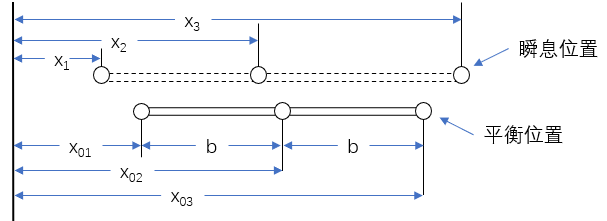
\includegraphics[scale=0.5]{./fig/4-2.png}
    \caption{描述线形三原子分子的坐标系}
\end{figure}

我们需要将势能写为位移坐标\footnote{作者没有在开始指明三个小球的质量,两端的小球质量为m,中间的小球质量为M。}。定义最左边质点的平衡位置为$x_{01}$,中心质点的平衡位置为$x_{02}$,最右边质点的平衡位置为$x_{03}$。
然后,定义位移坐标如下:
\[ 
\begin{array}{c}
    q_1=x_1-x_{01} \\
    q_2=x_2-x_{01} \\
    q_3=x_3-x_{01}
\end{array}
\]
因
\[b=x_{02}-x_{01}=x_{03}-x_{02}\]
故
\[V=\frac{k}{2}(q_2-q_1)^2+\frac{k}{2}(q_3-q_2)^2=\frac{k}{2}(q_1^2+2q_2^2+q_3^2-2q_1q_2-2q_2q_3)\]
现在我们可以写出势能的矩阵。矩阵元$v_{ij}$是势能表示式中项$q_iq_j$的系数。这意味着势能矩阵是
\[V=
\begin{pmatrix}
    k & -k & 0 \\
    -k & 2k & -k \\
    0 & -k & k
\end{pmatrix}
\]
动能比较简单些。在图4-2示出的坐标系中动能是
\[T=\frac{m}{2}(\dot{x}_1^2+\dot{x}_3^2)+\frac{M}{2}(\dot{x}_2^2)\]
若将位移坐标和它的时间导数代入此方程,可得
\[T=\frac{m}{2}(\dot{q}_1^2+\dot{q}_3^2)+\frac{M}{2}(\dot{q}_2^2)\]
也取$T$中的各项(此情况下只有三项),并放到矩阵中去,矩阵中的$t_{ij}$是$T$中$q_iq_j$的系数,可得出动能矩阵
\[T=
\begin{pmatrix}
    m & 0 & 0 \\
    0 & M & 0 \\
    0 & 0 & m
\end{pmatrix}
\]
特征值方程为
\[V\Phi=\omega^2T\Phi\]
需解的久期方程是
\[|V-\omega^2T|=0=
\begin{vmatrix}
    k-\omega^2m & -k & 0 \\
    -k & 2k-\omega^2M & -k \\
    0 & -k & k-\omega^2m
\end{vmatrix}
\]
用行的余因式很容易将久期行列式展开\footnote{这里对运算过程和结果的表示方法做了省略,不影响作者想表达的意思。}:
\[0=(k-\omega^2m)
\begin{vmatrix}
    2k-\omega^2M & -k \\
    -k & k-\omega^2m
\end{vmatrix}
+k
\begin{vmatrix}
    -k & -k \\
    0 & k-\omega^2m
\end{vmatrix}
=(k-\omega^2m)(\omega^2)[\omega^2Mm-k(M+2m)]
\]
其解为
\[\omega=\sqrt{\frac{k}{m}} \ ,\ 0 \ , \ \sqrt{\left(\frac{k}{m}\right)\left(1+\frac{2m}{M}\right)}\]

根据已发展的理论,特征值存在零解不被禁阻。我们只发现特征值$\omega^2$不能是负值。
如果读者返回去并考察理论在那个问题上的发展,他就可得出如下的结论,特征值$\omega=0$对应于其自由度的势能为零的某种运动。
具有零势能的体系并不是谐振子;它是无恢复力或反向力的某种运动。换句话说,它表示自由移动或自由转动。

这也是我们应该预期到的一点。前边我们用三个广义坐标描述此问题,但只应有两个坐标。
我们没有消去对应于与$x$轴平行的移动的广义坐标。这说明了一个重要问题,
非振动的分子运动若仍保留在被选取的广义坐标系中,则它的特征值$\omega^2$为零。

使用一组与振动联系着的只含二坐标的坐标系,我们能重新处理此问题。
为此,应写出我们希望禁阻的移动的方程,并用它来消除以前用的三个坐标$q_1,q_2,q_3$中的一个。
能够选取此方程的条件是使体系的质心在原点:
\[m(x_1+x_3)+Mx_2=0\]
进一步作下去可得到同样的非零特征值,但没有零特征值。

现在我们面临的问题是求简正振动的特征向量。为此,须将特征值(现为已知量)代回到特征值特征向量方程,解此方程求特征向量的分量。
每一特征值就有一特征向量,因此有几个特征值,此过程就要进行几\footnote{此处原文为“n”,与上文对不上,故改为"几"。}次。
振动问题和通常的特征向量问题不同,它不要求特征向量归一化为一,而要求$\bra*{\phi^i}T\ket*{\phi^i}=1$。
特征值方程为$V\Phi=\omega^2T\Phi$。第-次计算选取特征值$\omega^2=k/m$,得到
\[
\begin{pmatrix}
    k & -k & 0 \\
    -k & 2k & -k \\
    0 & -k & k
\end{pmatrix}    
\begin{pmatrix}
    \phi^1_1 \\ \phi^1_2 \\ \phi^1_3
\end{pmatrix}
=\frac{k}{m}
\begin{pmatrix}
    m & 0 & 0 \\
    0 & M & 0 \\
    0 & 0 & m
\end{pmatrix} 
\begin{pmatrix}
    \phi^1_1 \\ \phi^1_2 \\ \phi^1_3
\end{pmatrix}  
\]
将矩阵方程写成联立线性方程组
\[k\phi_1^1-k\phi_2^1=k\phi_1^1\]
\[-k\phi_1^1+2k\phi_2^1-k\phi_3^1=\frac{kM}{m}\phi^1_2\]
\[-k\phi_2^1+k\phi_3^1=k\phi_3^1\]
从第一个方程和最后一个方程得到
\[\phi^1_2=0\]
代入第二个方程得到
\[\phi_1^1=\phi_3^1\]
一个可接受的特征向量(在归一化以前) 是向$(a,0,-a)$。
需要与归一化类似的处理,$\bra*{\phi^i}T\ket*{\phi^i}=1$。以矩阵形式表示为:
\[
(a \ , \ 0 \ , \ -a) 
\begin{pmatrix}
    m & 0 & 0 \\
    0 & M & 0 \\
    0 & 0 & m
\end{pmatrix}
\begin{pmatrix}
    a \\ 0 \\ -a
\end{pmatrix}  
=  
\begin{pmatrix}
    a & 0 & -a
\end{pmatrix} 
\begin{pmatrix}
    ma \\ 0 \\ -ma
\end{pmatrix}  
=2a^2m=1
\]
所以,$a=1/\sqrt{2m}$。因此,归一化的特征向量为$(1/\sqrt{2m},0,-1/\sqrt{2m}$。

对特征值$\omega^2=(k/m)(1+2m/M)$,用同样过程给出未归一化的特征向量为$(a,-2ma/M,a)$
归一化的特征向量十分复杂,为
\[\left(\sqrt{\frac{M}{2mM+4m^2}},-\sqrt{\frac{4m}{4mM+2M^2}},\sqrt{\frac{M}{2mM+4m^2}}\right)\]
特征值$\omega^2=0$的特征向量也可以计算,未归一化的特征向量为$(a,a,a)$;归一化的特征向量的每个分量为$1/\sqrt{2m+M}$。

做为对振动问题的解的最后验证,我们对非对角型的$V$矩阵和对$T$矩阵实施变换。
结果应给出,$V$矩阵变换成以特征值$\omega^2$为对角元的对角矩阵,$T$矩阵变换为单位矩阵。

为简便计,考虑三原子线形分子,如$N_3^-$或$I_3^-$,因而$m=M$。
特征向量为
\[\left(\sqrt{\frac{1}{2m}},0,-\sqrt{\frac{1}{2m}}\right) \ , \ 
\left(\sqrt{\frac{1}{6m}},-\sqrt{\frac{2}{3m}},\sqrt{\frac{1}{6m}}\right) \ , \ 
\left(\sqrt{\frac{1}{3m}},\sqrt{3m},-\sqrt{\frac{1}{3m}}\right)\]
可用图解法解释这些特征向量。特征向量$(1/\sqrt{2m},0,-1/\sqrt{2m})$表示当最左边的原子向左移动时,最右边的原子向右移动,或相反。
这叫做振动的对称伸长方式,示于图4-3a。另一方面,特征向量$(1/\sqrt{6m},-2/\sqrt{6m},1/\sqrt{6m})$表示端原子(1和3)朝同方向运动,而中心原子(2)朝相反方向运动。
中心原子移动的距离为端原子移动距就的二倍以保持质心不变。这叫做反对称伸长方式,示于图4-3b。

最后一个特征向量$(1/\sqrt{3m},\sqrt{3m},-1/\sqrt{3m})$不保持质心固定。事实上此特征向量对应于分子的匀速移动。这是对应于特征频率为零的特征向量。

\begin{figure}[htbp]
    \centering
    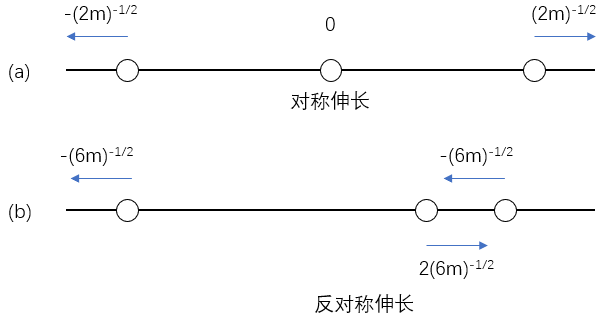
\includegraphics[scale=0.5]{./fig/4-3.png}
    \caption{线形三原子分子的振动的简正方式}
\end{figure}

\section{刚性力学体系的转动}
在上节中我们发展了振动力学体系的运动方程,并证明那种分析如何用到分子振动。
在本节中要发展转动力学体系的运动方程,并要证明如何应用于分子转动。
如上节末指出那样,有比这里介绍的方法更优异的方法可用;下边的讨论只是对一般问题作一概述。

对力学体系可求拉格朗日方程(方程4-31)的解,方程中的拉格朗日函数是按方程4-30定义。
对$V=0$因而$L=T$的刚性体系\footnote{刚性分子骨架的假定自然是不正确的,因分子确在振动,然而此假定可使讨论简化,并能使一些有兴味的概念显现出来。同样地,对阻尼转动这一非常有兴味的情况假定$V=0$也是不正确的。}
的转动拉格朗日函数特别简单。

刚性转动的动能的形式也特别简单。因为按定义
\[T=\frac{1}{2}\sum_im_iv_i^2 \tag{4-62}\]
故需对转动的$v_i$加以说明。简单的图可使同学们确信,对于圆周运动
\[\mathbf{v}_i=\omega \times \mathbf{r}_i \tag{4-63}\]
式中$\omega$是角速度。在一般情况下方程4-63成立。应用方程4-63,则方程4-62变为
\[T=\frac{1}{2}\sum_im_i\mathbf{v}_i \cdot (\omega \times \mathbf{r}_i) \tag{4-64}\]
可以证明方程4-64的乘积中的向量的顺序可以改变,给出
\[T=\frac{\omega}{2}\sum_im_i(\mathbf{r}_i \times \mathbf{v}_i)=\frac{\omega}{2}\sum_i\mathbf{l}_i=\frac{1}{2}\omega \cdot \mathbf{L} \tag{4-65}\]
式中$\mathbf{l}_i$是第$i$个质点的角动量,$\mathbf{L}$是整个体系的角动量。

而
\[\mathbf{L}=\sum_im_i(\mathbf{r}_i \times \mathbf{v}_i)=\sum_im_i(\mathbf{r}_i \times (\omega \times \mathbf{r}_i))=\sum_im_i(\omega\mathbf{r}_i^2-\mathbf{r}_i(\mathbf{r}_i-\omega)) \tag{4-66}\]
使用转动惯量张量的定义可将方程4-65改写成简缩的形式。
\begin{definition}[转动惯量张量]
    绕某一点转动的物体的转动惯量张量是一对称矩阵,在笛卡儿坐标系里定义如下。
    令$q_1^v,q_2^v,q_3^v$号为质点的$x,y,z$坐标。转动惯量的$i,j$元定义为:
    \[I_{ij}=\sum_pm_p(\mathbf{r}_p^2\delta_{ij}-q_i^vq_j^v) \tag{4-67}\]
    式中$\mathbf{r}_p$是质点$P$与特定点的距离。
\end{definition}

用$I$的这个定义可写出
\[\mathbf{L}=\mathbf{I}\omega \tag{4-68}\]
因此
\[T=\frac{1}{2}\omega \cdot \mathbf{I}\omega=\frac{1}{2}\bra*{\omega}\mathbf{I}\ket*{\omega} \tag{4-69}\]
现在摆在我们面前的问题是怎样精确地解释转动动能公式中的转动惯量张量的作用。

在4-1节中我们学过质点体系绕点转动的角动量,可分解为各质点绕质心转动的角动量加质心的角动量。
因此,如果我们只将注意力集中在分子的转动上,即如果我们为分子取的坐标系是使质心固定不动,则角动量就是绕质心转动的角动量。
于是方程4-67中的$\mathbf{r}_p$可取为质心到质点$p$的距离。

若选的坐标系可能使$\mathbf{I}$是对角的,如为$\xi,\eta,\varsigma$坐标系,则动能可取特别简单的形式
\[T=\frac{\omega \cdot \mathbf{I}\omega}{2}=\frac{1}{2}\left(\mathbf{I}_{\xi\xi}\omega_{\xi}^2+\mathbf{I}_{\eta\eta}\omega_{\eta}^2+\mathbf{I}_{\varsigma\varsigma}\omega_{\varsigma}^2\right) \tag{4-70}\]
式中$\mathbf{I}_{\xi\xi},\mathbf{I}_{\eta\eta},\mathbf{I}_{\varsigma\varsigma}$是$\mathbf{I}$的三个对角元,
$\omega_{\xi},\omega_{\eta},\omega_{\varsigma}$是角速度向量的分量。

$\mathbf{I}$能对角化吗?能,因为$\mathbf{I}$是对称的和实的。当$i \neq j$时,
\[\mathbf{I}_{ji}=\sum_p(-m_pq_i^pq_j^p)=\sum_p(-m_pq_j^pq_i^p)=\mathbf{I}_{ji} \tag{4-71}\]
因$\mathbf{I}$是厄米矩阵,故可求助于3-4节中有关厄米算符的特征值的定理。
因此,称为主转动惯量的$\mathbf{I}$的特征值是实的,称为主轴的特征向量是正交归一的。
联系任意笛卡儿轴系和主轴系的相似变换称为主轴变换。如将$\mathbf{I}$的矩阵对角化,我们马上就可使用$T$的更简单的表示式(方程4-70)来讨论刚性转子的能量。

对刚性转子,习惯上是按等价主转动惯量的数目命名如下
\footnote{为方便打表对原书下表稍作修改。}:
\[
\begin{tabular}{c|c}
    \hline
    等价转动惯量数量 & 转子名称 \\ \hline
    3 & 球陀螺 \\
    2 & 对称陀螺 \\
    none & 非对称陀螺 \\
    \hline
\end{tabular}
\]

\textbf{例}

计算水的主转动惯量。若水分子的取向如图4-4示出的坐标系中那样,则容易算出在此坐标系中转动惯量张量质心在原点的矩阵元。
应注意,分子的取向对称于位于坐标系原点的质心。我们必须先计算可给出分子图4-4水分子的主轴的几何形状的核的位置。
因为质心在原点,故此计算可用简单的三角学和质心的方程
\[\sum_im_i\mathbf{r}_i=0\]
核的位置是\footnote{书上氢原子的坐标还少了负号(emmm}
$\mathbf{r}(0)=(0.00,0.07),\mathbf{r}(H_a)=(-0.76,-0.55),\mathbf{r}(H_a)=(0.76,-0.55)$:
$|\mathbf{r}(0)|=0.07,|\mathbf{r}(H_a)|=|\mathbf{r}(H_b)|=0.94$。
应用方程4-67,可计算出水绕质心转动的转动惯量张量。例如,
\[\mathbf{I}_{xx}=\sum_pm_p(\mathbf{r}^2_p-x_p^2)=[16(0.0049-0.0000)+1(0.881-0.578)+1(0.881-0.578)](M)(10^{-16})\]
\[=1.21 \times 10^{-40}g \cdot cm^2\]
式中M是质子的质量$1.67 \times 10^{-24}g,1\AA^2=10^{-16}cm^2$。同样地
\[\mathbf{I}_{xy}=-\sum_pm_px_py_p=-[(16)(0)(0.07)-(1)(-0.76)(-0.55)-(1)(0.76)(-0.55)](M)(10^{-16})=0\]
用类似的办法可计算出张量$\mathbf{I}$
\[\mathbf{I}=
\begin{pmatrix}
    1.21 \times 10^{-40} & 0 & 0 \\
    0 & 1.93 \times 10^{-40} & 0 \\
    0 & 0 & 3.08 \times 10^{-40}
\end{pmatrix}
\]
因张量是对角化的矩阵,故立刻就可求出主转动惯量。我们还可求出,图4-4上的$x,y,z$轴是主轴。
\begin{figure}[htbp]
    \centering
    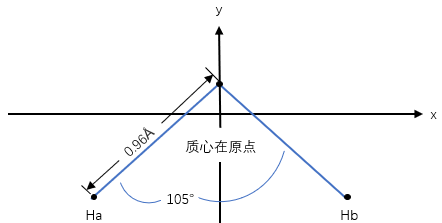
\includegraphics[scale=0.5]{./fig/4-4.png}
    \caption{水分子的主轴}
\end{figure}

这种分子分类和用矩阵代数求主转动惯量的方法在前一节中已发挥了促进作用。

\begin{problemset}
\item 证明方程4-3下边所讲的有关叉乘的性质。
\item 证明在4-1节中提出的质点系的三个守恒定理。
\item 证明在4-1节中提出的三个分离定理。
\item 用一刚性、无重、长度为$l$的棒将质量为$m$的二质点联结起来;棒的中心在用金属丝围成的半径为$a$的圆环上作无摩擦的运动。选用适合的简单的广义坐标组,并用此坐标组将$T$表示出来。
\item 写出在三维空间运动的摆的拉格朗日方程;用刚性的、无重的榜悬挂的质量为$m$的质点在重力的作用下运动。
\item 用一弦(无重、非弹性)将质量不等的二质点联结起来。一质点放在桌子上,另一质点放在桌子一边滑动(无摩擦)。用拉格朗日力学描述此运动。
\item 由弹簧将一质量为$m$的球联于平滑台的中心。弹簧的力常数为$k$,平衡长度为$r$。求体系的运动方程,并加说明。
\item  (a)推导方程4-23a;(b)推导方程4-23b。
\item 一质点在矩形箱内由四个弹簧拉住,每两个弹簧的力常数相同。让质点离开平衡位置一小的位移。描述其运动。
\item 推导方程4-53。
\item 重新推导4-3节的例中提示的用质心坐标系表示的线形三原子分子的简正方式的公式。
\item 求水分子振动的简正方式和频率。
\item 求二氧化碳分子振动的简正方式和频率。
\item 推导方程4-63,4-65和4-66。
\item 证明欧拉定理:有一点固定的刚体的最一般的位 移是绕其轴转动。
\item 计算4-4节的例中水的转动惯量张量,但取另一坐标系;氧原子在原点,-O-H键在$x$轴上。将计算结果和例中的结果比较。
\item 分子$CCl_4, NCl_3,OCl_2,FCl$都是第二周期元素的氯化物。计算每一分子的主转动惯量,并按“陀螺”的特殊种类分类,对每个分子划出简图,并示出其主轴。应查阅这些分子的结构。
\item 证明正四面体和立方体分子是“球顶”。
\end{problemset}